\chapter{Marco teórico}
\label{cap:marco_teorico}
	En este capítulo se explicarán de manera resumida los conceptos y tecnologías más importantes relacionadas con el desarrollo del proyecto, así como una breve introducción a la monitorización de redes.\\\\
	
	A continuación, se describirán las soluciones y propuestas empleadas para resolver el problema sobre la red de transporte. Así mismo, se explicarán los estándares y protocolos utilizados y más destacados. En concreto se hablará de las tecnologías inalámbricas: WiFi tanto para cortas distancias como para larga distancia (WiLD), WiMAX, LTE, \textit{Television White Spaces} (TVWS) y los protocolos propietarios de Mikrotik \cite{Mikrotik} Nstreme y NV2.\\
	De igual forma se detallará la legislación y normativa vigente en el marco del proyecto respecto al uso y despliegue de dichas tecnologías, acorde con el artículo \cite{espinoza2018wireless}.\\\\
	
	Por último, se analizarán diferentes programas software de monitorización y gestión de redes que es razonable utilizar en este proyecto, estableciendo una comparativa entre ellos. Del mismo modo, se comentará de manera más detallada el funcionamiento y características de la herramienta escogida como solución para el desarrollo del proyecto.
	
\section{Red de transporte en redes inalámbricas para zonas rurales}
	Como ya se ha comentado, la extensión de la cobertura de redes de telecomunicaciones en zonas rurales tropieza con el hándicap del elevado coste de despliegue de las infraestructuras necesarias frente a una expectativa de bajo retorno de la inversión, debido a la escasa densidad de población de estas zonas; este problema es mayor cuanto menor es la densidad de población, mayor la distancia focos de concentración, y menor el poder adquisitivo de la población. Por tanto, existe la necesidad de soluciones flexibles y de bajo coste para tratar de resolver dicho problema.\\\\
	
	En lo que respecta a redes de acceso radio a comunicaciones móviles de banda ancha, una solución que se ha aplicado en algunos proyectos, como es el caso del TUCAN3G, es el uso de de femtoceldas. Las femtoceldas son estaciones base diseñadas para servir a un reducido número de usuarios concurrentes y con una potencia de transmisión también muy pequeña, y se asume que usan como backhaul un enlace de acceso a Internet preexistente; en un principio estaban diseñadas para cubrir los huecos de cobertura existentes en determinadas zonas, por lo cual muchas de ellas están alojadas dentro de edificios. Lo que hace de las femtoceldas una solución viable es su escaso consumo energético y su flexibilidad. Esto aporta una solución más viable para el operador de telefonía frente al uso de nodos convencionales: la inversión es menor obteniendo un redimiento equitativo.\\\\
	
	Por otra parte, para transportar el tráfico intercambiado entre estas redes de acceso y la red fija de transporte del operador, hace falta también una solución igualmente apropiada para el transporte rural. Se requieren tecnologías de muy bajo costo y flexibles para que al operador le traiga cuenta desplegar tal infraestructura, o incluso compartirla con otros agentes socioeconómicos. A continuación se procede a explicar brevemente el funcionamiento de las distintas tecnologías pertenecientes al ámbito de comunicaciones inalámbricas para enlaces de larga distancia, obteniendo así diferentes rendimientos de la solución propuesta.


\section{Protocolos Inalámbricos}

		\subsection{Nstreme}
		El protocolo Nstreme es un protocolo inalámbrico, que posteriormente daría lugar al protocolo NV2, que utiliza Polling como protocolo de acceso al medio correspondiente a la capa MAC. El funcionamiento del protocolo viene ilustrado en la imagen \ref{Nstreme} como protocolo de acceso al medio correspondiente de la capa MAC. Siguiendo este protocolo, la comunicación entre estaciones base se produce de manera independiente a la comunicación con los nodos cliente. La comunicación entre clientes y estaciones base se realiza utilizando mensajes de señalización, o tokens, con los que las estaciones base conocen el comienzo y final de la transmisión. Si la estación base considera que un nodo cliente no está emitiendo pasaría a inspeccionar otro nodo de la red.    
	
		\begin{figure}[H]
			\centering
			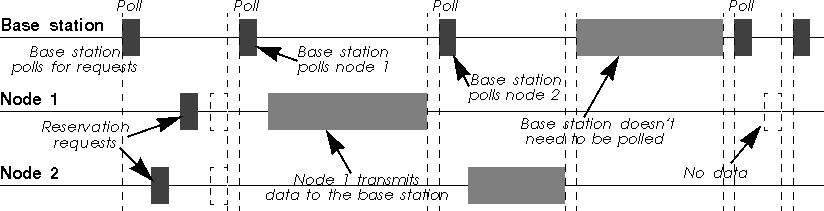
\includegraphics[width=0.7\textwidth]{img/Polling.png}
			\caption{Funcionamiento \textit{Polling} en Nstreme}
			\label{Nstreme}
		\end{figure}
		
		Acorde con esto, las ventajas e incovenientes del protocolo son:
		\begin{itemize}
			\item No existen limitaciones entre estación base y cliente.
			\item Baja sobrecarga de cabeceras en las tramas por lo que permite conseguir mayores tasas de envío.
			\item Retardo por propagación y latencia como consecuencia de usar \textit{Polling}.
		\end{itemize}

		\subsection{NV2}
		El protocolo NV2 es un protocolo inalámbrico, perteneciente a la capa MAC \cite{MacLayer}, basado en el acceso múltiple por división de tiempo (TDMA) en lugar de \textit{Polling} o acceso múltiple con escucha de señal portadora (CSMA). Este último es el usado más comúnmente por la mayoría de equipos relacionados con el estándar 802.11.\\\\
		
		Para explicar el funcionamiento del protocolo NV2, mostrado en la figura \ref{NV2}, vamos a suponer un escenario en el cuál nuestra red estará compuesta por una estación base (BS), la cuál está utilizando el protocolo NV2, y diferentes clientes que comparten BS. El acceso al medio de los clientes estará organizado por la BS, que dividirá el tiempo en períodos. Estos períodos estarán dinamicamente divididos en porciones para \textit{Downlink} (datos enviados desde la BS hacía el cliente) y \textit{Uplink} (datos enviados desde el cliente a la BS). Al comienzo de cada período, la BS mandará un mensaje mediante \textit{broadcast} a los clientes con información sobre en qué momento han de transmitir y del tiempo disponible para ello. \\
		Acorde con lo anterior, la BS de manera periódica asigna una parte del tiempo de Uplink para un ''cliente desconocido''. Dicho tiempo tiene como objetivo favorecer la integración y comunicación de un nuevo cliente con la red (si lo hubiera). Para ello, la BS estima el retardo que existe entre la misma y el nuevo cliente reajustando el tiempo de Uplink, permitiendo completar el registro y comunicación del nuevo cliente con la red.
		
		\begin{figure}[H]
			\centering
			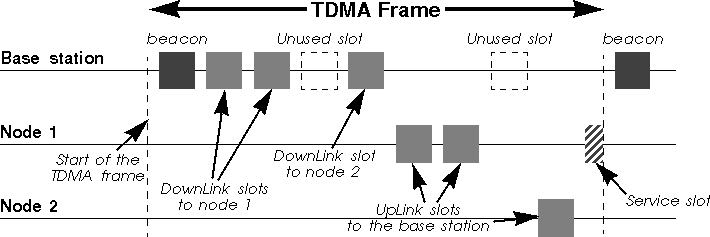
\includegraphics[width=0.7\textwidth]{img/TDMA.png}
			\caption{Funcionamiento TDMA en NV2}
			\label{NV2}
		\end{figure}
		
		Las ventajas e inconvenientes del protocolo NV2 se detallan a continuación:
		\begin{itemize}
			\item Mejor rendimiento en redes punto a punto (PTP).
			\item Mayor \textit{throughput} y menor latencia.
			\item No existe el problema del nodo oculto.
			\item Únicamente se podrán establecer redes homogéneas al protocolo NV2, en consecuencia podrá existir interferencia entre redes que no usen NV2 y viceversa.
		\end{itemize}
		
\section{Tecnologías Inalámbricas}
Antes de comenzar con el análisis sobre las diferentes tecnologías inalámbricas estudiadas en el marco del proyecto,  debemos de tener en cuenta todas la limitaciones existentes en el proyecto Napo. Esto implica, no sólo el coste e inversión económica que ha de hacerse para desarrollar una infraestructura de telecomuniaciones viable, si no que también debemos tener en cuenta las normas y legislaciones existentes en cuanto al uso del espectro radioeléctrico peruano.\\\\

Durante las últimas décadas, las telecomunicaciones en toda sudámerica y en especial en áreas rurales han sufrido fuertes barreras y obstáculos frente a la implantación de un modelo de desarrollo sostenible. Como resultado de esto, el empobrecimiento de la población y pérdida de calidad de vida fue en aumento. La vida social en zonas rurales se distanció aún más de la existente en las urbes, provocando así el aumento de ausentismo escolar y tasa de mortalidad. Para tratar de combatir esto, desde varios gobiernos sudamericanos se promovió la importancia de trazar nuevos caminos y estructuras para tratar de apaliar el déficit existente en dichas zonas rurales.\\\\

Como cosecuencia de esto, en 2005 el ministerio peruano de transporte y comunicaciones (CTM), aprobó una nueva ley sobre el uso del espectro radioeléctrico a nivel nacional. Con el objetivo de utilizar dicho espectro de forma más eficiente y promover el despliegue de nuevas redes inalámbricas, se redefinieron los usos y asignaciones de las bandas disponibles en el espectro, tratando de satisfacer así la fuerte demanda creciente en cuanto a servicios TIC. \\\\

El objetivo final de invertir en una ampliación de la infraestructura de telecomunicaciones ya existente era ofrecer servicios mínimos de acceso público a instituciones públicas, como por ejemplo escuelas, puestos de salud, comisarías, etc... Para tratar de llevar a cabo dicha labor se escogió las tecnologías inalámbricas como solución a dicho problema, ya que permiten una mayor flexibilidad, requieren una inversión inicial de capital menor meintras que su despliegue y desarrollo es más rápido, y por último son tecnologías más eficientes en términos de operación y gestión de redes.\\\\

A continuación, analizaremos el espectro readioeléctrico en el contexto peruano, así como el uso, aplicación y evolución de las diferentes tecnologías que han sido objeto de estudio durante la realización de este Trabajo Fin de Grado.

\subsection{WiFi}
La tecnología WiFi surge como solución a los problemas que estaban surgiendo en relación a las redes inalámbricas locales (WLAN). Desde su primera versión, el estándar 802.11a hasta la versión actual 802.11n, esta tecnología ha sido utilizada como solución a los problemas de comunicaciones inalámbricas para redes metropolitanas y redes rurales con cierta extensión debido a sus características. La principal característica de WiFi es su mecanismo de acceso al medio basado en CSMA/CA (\textit{Carrier Sense Multiple Access/Collision Avoidance}) perteneciente a toda la familia de CSMA cuya principal diferencia es la forma de repartir el canal compartido para una estación que desea transmitir. El funcionamiento de CSMA se basa en la búsqueda de una portadora reconocida en el medio compartido para otorgar el turno de transmisión a la estación cliente, evitando así colisiones entre estaciones que tienen en curso una transmisión y estaciones que desean empezar a transmitir. La variante CSMA/CA está optimizada para canales radio minimizando así el problema de colisiones múltiples.\\\\

Gracias a el avance del estándar las tasas registradas para esta tecnología pueden alcanzar los 600 Mbps teóricos y los 300 Mbps de cobertura, esto implica la inclusión de un nuevo término HT-STA (\textit{High Throughput STAtion}), el cual se diferencia de las non-HT-STA en los mecanimos de las capas PHY y MAC.\\
Por un lado, en la capa MAC los cambios respecto a las estaciones non-HT-STA son referentes a la agregación de tramas, uso de protocolo de dirección inversa, reducción de tiempos de espera y mecanismos de coexistencia con non-HT-STA. Por otro lado, en la capa PHY la principal mejora es la introducción y soporte de MIMO que permite la multiplexación espacial. \\\\

A continuación se detallan nuevas mejoras y técnicas aplicadas al estándar 802.11n, con el objetivo de mejorar las prestaciones y eficiencia del mismo acorde con las estaciones HT:
\begin{itemize}
    \item Ampliación del espectro de 20 MHzs a 40 MHzs, agrupando canales consecutivos de 20 MHzs y considerando de 1 MHzs el tamaño de las bandas de guarda, lo que permite duplicar la información contenida dentro del canal.
    
    \item Dualidad de canales a la hora de seleccionar una frecuencia de trabajo u otra , es decir, utilizar las frecuencias de 2,4 y 5 GHzs indistintamente permitiendo así que exista retrocompatibilidad con todas las versiones de WiFi.
    \item Mejora de agregación de tramas sobre capa MAC basada en la agrupación global de tramas mediante las técnicas de A-MDSU (\textit{Aggregate MAC Service Data Unit}) y A-MPDU (\textit{Aggregate MAC Protocol Data Unit}). \\
    Por un lado, la técnica A-MDSU se aplica al inicio de la capa MAC y consiste en agregar múltiples MSDU (\textit{MAC Service Data Unit}) como primer paso al formar la trama totalitaria MPDU (\textit{MAC Service Data Unit}). Por otro lado, la técnica A-MPDU se efectua al final de capa MAC agregando múltiples MPDU (\textit{MAC Protocol Data Unit}) transportadas como una simple PSDU (\textit{Protocol Service Data Unit}) por la capa PHY.\\
    En conclusión, el uso de estas técnicas permite reducir la transmisión de cabeceras debido a que la trama de datos será enviada en una única transmisión, utilizando el medio compartido de forma más eficiente.
    
    \item Transmisiones múltiples sin necesidad de esperar un tiempo excesivo reduciendo el acceso total al medio y aumentando la eficiencia de la red. Para esto se utilizan los mecanismos de RIFS (\textit{Reduced InterFrame Space}) y SIFS (\textit{Short InterFrame Space}).
    
    \item Modulación y codificación determinada por los equipos para establecer comunicación entre ellos. Definimos MCS (\textit{Modulation and Coding Schema}) como el esquema existente en los equipos para comunicarse a través de una modulación determinada. Actualmente, existen 127 MCS para el estándar 802.11n, no obstante en este Trabajo Fin de Grado sólo han sido utilizadas las MCS comprendidas entre MCS8 y MCS15 destinadas a diversidad espacial en transmisión 2x2 (MIMO 2x2).
\end{itemize}

\subsubsection{WiLD: WiFi para largas distancias}
Como hemos comentado en el apartado anterior, WiFi utiliza el protocolo CSMA/CA para acceder al medio lo que implica que no sea del todo satisfactorio en el ámbito de comunicaciones inalámbricas de largo alcance, ya que los tiempos de silencio en el canal necesarios para esta clase de control de acceso al medio se hacen insuficientes para evitar las colisiones o, si se agrandan fuera de lo que marca el estándar, tienen un alto impacto en la eficiencia. No obstante, esto no hace que el uso de WiFi se deseche por completo ya que, realizando un pequeño ajusta al funcionamiento del protocolo de acceso al medio y asegurando una linea de visión directa entre los enlaces conseguiremos una solución viable en nuestro contexto.\\\\
		
WiFi es usado principalmente en canales cuyo ancho de banda se corresponde a 20 MHz. Sin embargo, su uso para canales de 5 y 10 MHz es también posible desde las primeras versiones del estándar, y a partir de la revisión IEEE 802.11n es también posible emplear canales de 40 MHz. Adicionalmente, desde IEEE 802.11n la transmisión y recepción de señal existiendo diversidad espacial es posible, ya que la mayoría de equipos están diseñados con antenas duales MIMO 2x2. Otra característica que ofrece WiFi es su funcionamiento respecto a la agregación de tramas, ya que podemos crear una trama de mayor tamaño manteniendo una única cabecera y siendo capaces de establecer una diferenciación en el tráfico. \\\\
		
Aunque el estándar ofrece mejoras en la capa física, tendremos que tener en cuenta otros parámetros como la potencia de señal recibida (SNR), la modulación y códigos utilizados para obtener una tasa de transmisión óptima en nuestra red. Teniendo en cuenta todo esto, WiFi podría ser una solución viable y sostenible en el marco de nuestro proyecto. Sin embargo, debemos tener en cuenta el rendimiento que ofrece el estándar frente al canal utilizado y su gestión de acceso al medio. Del mismo modo, hay que tener en cuenta la gran distancia existe entre las estaciones y la diversidad climotológica existente a lo largo de la red.\\\\

Acorde con el artículo \cite{simo2014assessing}, vemos como el rendimiento de WiFi en largas distancias no es del todo óptimo, debido a su uso de CSMA/CA como protocolo de acceso al medio. Por ello, se propone realizar un ajuste en el protocolo y utilizar TDMA. Así obtendremos una mayor eficiencia y evitando contiendas en el medio que resultan muy ineficientes en distancias largas. Independientemente del protocolo utilizado en la capa MAC, cualquier \textit{hardware} que utilice el estándar 802.11 tendrá las características mencionadas anteriormente. Por tanto, la cuestión es obtener un equilibrio en cuanto a despliegue y rendimiento. Por un lado, deberemos garantizar la línea de visión directa entre radioenlaces de nuestra red, y por el otro lado deberemos proponer una solución viable en lo que a inversión en estructura y equipos se refiere.\\\\

\subsubsection{Marco legislativo}
En 2008 el CTM alojó las bandas destinadas a la tecnología WiFi en las siguientes frecuencias: 902-928 MHzs, 2,4-2,483.5 GHzs, 5,725-5,850 GHzs, 5,250-5,350 GHzs y 5,470-5,725 GHzs. Dichas bandas estaban destinadas a los servicios de telecomunicaciones en zonas rurales y áreas en las cuáles no se requería el uso de banda licenciada. \\\\

De igual forma, durante el 2011 y hasta el 2013 está legislación sufrió algunas actualizaciones, conviertiendo la banda de 902-915 MHzs en una banda licenciada para el uso de servicios de telecomunicaciones. Por tanto, el CTM tuvo que reestructurar está repartición del espectro. Dicho rediseño se llevó a cabo en 2013 como resultado, el reparto de espectro quedó de la siguiente manera: 915-928 MHz, 916-928 MHz, 2,400-2,483.5 GHzs, 5,725-5,850 GHzs, 5,250-5,350 GHzs y 5,470-5,725 GHzs.\\\\

El CTM redistribuyó el espectro radioeléctrico en consecuencia de la fuerte demanda de servicios de telecomunicaciones existentes. Dicha reforma garantizaba la viabilidad de los servicios en redes ya esxistintes, y promovía el despliegue de nuevas redes que aportarán una solución frente a la fuerte demanda existente. El uso de banda no licenciadas era un factor clave a la hora de rehacer esta distribución, ya que los operadores de telefonía no percibían ningún tipo de coste si utilizaban dichas bandas.\\\\

		
\subsection{WiMAX}
El estándar IEEE 802.16, más comunmente conocido como WiMAX, fue diseñado para su uso en áreas metropolitanas, aunque debido a su funcionamiento existe la posibilidad de utilizarlo en áreas rurales que utilizan banda ancha. Si bien el estándar IEEE 802.16 especifica el uso de esta tecnología en distintas bandas de frecuencias, y uno de los perfiles es para bandas no licenciadas en 5 GHzs, el consorcio de empresas conocido como WiMAX Forum, responsable de certificar la compatibilidad e interoperabilidad de productos en el marco de este estándar, no ha reconocido un perfil para bandas no licencias. Por lo tanto, existen equipos IEEE 802.16 que funcionan en banda libre de 5 GHz, pero formalmente no podrían usar la denominación WiMAX. El protocolo de acceso al medio de este estándar es TDMA y la técnica de transmisión utilizada es OFDM.\\\\

La capacidad óptima en un radioenlace que utiliza WiMAX depende entre otros factores, de la modulación que se consiga transmitir, la codificación utilizada, el tamaño de la trama que deseemos enviar y el intervalo de guarda existente entre los símbolos OFDM. Acorde con el artículo \cite{simo2014assessing} las tasas obtenidas si utilizamos WiMAX en enlaces de larga distancia, pueden estar comprendidas entre 1.6 Mbps y 33 Mbps, teniendo en cuenta un envío de 20 tramas por milisegundo. Estos resultados de diversidad y ganancia espacial son similares a los obtenidos con WiFi. \\\\
		
Aunque los sistemas de comunicaciones que utilizan los estándares 802.11 y 802.16 en bandas no licenciadas tienen un bajo coste, tanto por el precio de los equipos como por la posibilidad de utilizar el espectro sin pagar licencias, su despliegue si entraña costes nada desdeñables por el diseño y construcción de estructuras de soporte para ubicar los sistemas de comunicación y las antenas a las elevaciones necesarias para enlaces de largas distancias, con el objetivo de mantener línea de visión directa. Dependiendo del contexto geográfico y de la distancia focos de concentración de población, la instalación de estas estructuras de soporte pueden ser un coste muy dominante que hagan muy costoso el despliegue de las infraestructuras de transporte con independencia del equipamiento de comunicaciones usado. Aparte de esto, la transmisión de potencia en bandas no licenciadas se debe tener en cuenta, pues existen restricciones de límites de potencia, lo que condicionan la viabilidad de nuestros enlaces.

\subsubsection{Marco legislativo}
En el año 2005 y con el objetivo de mejorar el acceso a los servicios de telecomunicaciones mínimos, el CTM destinó las bandas de 3,4-3,5 GHzs y 3,5-3,7 GHzs (también conocidas como bandas 3,4) para dicho objetivo. Aparte de este reparto, el MTC dictaminó que los operadores que quisieran obtener un canal en las bandas ya mencionadas deberían limitarlo a un tamaño máximo de 50 MHzs, independientemente del área geográfica en cuestión.\\\\

En el 2006 este espectro volvió a sufrir otro rediseño, dejando las bandas comprendidas entre las frecuencias de 2,5-2,692 GHzs para el acceso público a servicios mínimo de telecomunicaciones. Dicho rediseño trajo consigo una subasta de parte del espectro por parte del MTC, garantizando el uso de bandas libres de impuestos en Lima. A lo largo de 2007, el MTC se dio cuenta que dichas bandas tenían un gran potencial en cuanto a rentabiliadad y rendimiento, por lo tanto decidieron dedicar esas bandas a mejorar el uso de servicios móviles mediante el uso de WiMAX.\\\\

Este último hecho no suponía una tarea sencilla, ya que parte del espectro tenía que volver a ser restructurado y esto implicaba una inversión económinca adicional para recuperar la licencia de las bandas antes mencionadas. Con el objetivo de ampliar la infraestructura de redes y mejorar el acceso a las ya existentes, en 2010 se llevó a cabo otra reestructuración del espectro. Esto implicó una inversión de capital adicional ya que muchas bandas habían sido licenciadas.

\subsection{LTE}
La tecnología LTE (\textit{Long Term Evolution}) es un estándar para comunicaciones inalámbricas de transmisión de datos a alta velocidad para terminales de datos y dispositivos móviles. Esta tecnología pertenece al grupo de tecnologías englobadas dentro del 3GPP (\textit{The 3rd Generation Partnership Project}) cuyo principal objetivo es ofrecer acceso inalámbrico a servicios móviles, dentro de esta familia destacan los estándares GSM(\textit{Global System for Mobile communications}) de segunda generación y UMTS (\textit{Universal Mobile Telecommunications System}) clasificado de tercera generación. El estándar UMTS fue diseñado como evolución de GSM y aparte de obtener una mayor tasa de transmisión, su principal diferencia es la utilización del medio ya que UMTS utiliza W-CDMA (\textit{Wideband Code Division Multiple Access)} como protocolo de acceso al medio.\\\\

Como siguiente paso en el proceso evolutivo de dichas tecnologías aparece LTE cuyas prestaciones mejoran respecto a los anteriores estándares, ya que su principal diferencia es el protocolo de acceso al medio, que este caso es OFDM. Este cambio implica aumentar la tasa de transmisión instántanea a valores de 100 Mbps en el \textit{downstream} y 30 Mbps en el \textit{upstream}.\\
El siguiente paso en lo que a este estándar se refiere es el denominado LTE-A (\textit{LTE Advanced}) que ofrece tasas de transmisón mucho mayores en enlaces radio y una mejora en la arquitectura de LTE.

\subsubsection{Marco legislativo}
Desde 2005 el MTC permitía a los operadores de telecomuniaciones adquirir bandas licenciadas con un máximo de 60 MHzs para ofrecer sus servicios. Dicho modelo estaba enfocado a mantener la viabilidad y competitividad en el mercado de las telecomunicaciones, en cuanto al acceso público a redes. El espectro que se ofertaba y el que era accesible por parte de las operadoras era el comprendido entre 700, 800, 900 y 1900 MHzs. En 2010, este espectro fue identificado como una barrera para el desarrollo e implementación de acceso a nuevas redes, tanto en un entorno urbano como en un entorno rural.Como resultado de esto, se estableció un nuevo plan de políticas y regulaciones con el objetivo de maximizar el rendimiento del espectro actual teniendo en cuenta la aparición de nuevas tecnologías y las exigencias del mercado de las telecomunicaciones.\\\\

En el 2011,  por un lado las operadoras ofrecían sus servicios de acceso a la red en las bandas de 800 y 1900 MHzs y por el otro, el MTC alojaba badnas adicionales para promover el acceso a nuevos servicios públicos de telecomunicaciones. Dichas bandas son las siguientes: 894 - 902 MHzs, 939-947 MHzs, 902-915 MHzs, 947-960 MHzs 1,710 - 1,770 GHzs, 2,110 - 2,170 MHzs, 902-915 MHzs y 947-960 MHzs. Todas estas bandas fueron subastadas a las operadoras, lo que manifestaba una creciente demanda en cuanto al desarrollo de nuevas redes de acceso utilizando nuevas tecnologías.\\\\

En 2013 el MTC realizó una modificación en la regulación de uso del espectro. Esta nueva regulación estaba enfocada a modificar los 60 MHzs que imponían a las operadoras, ya que en muchos casos se estaba alcanzando e incluso sobrepasando dicha capacidad. Para ello, se mantuvo el uso de 60 MHzs en las bandas de 800, 900 y 1900 MHzs mientras que en las bandas de 1,7 y 2,1 GHzs se ofertaban 80 Mhzs en total, divididos en dos franjas de 40 MHzs ubicadas cada una de ellas en diferentes partes del espectro. El uso creciente de tecnologías 4G-LTE provocó que el MTC subastará dos bloques dedicados en las bandas de 1,7 y 2,1 GHzs para dichas tecnologías.

\section{Gestión del tráfico y QoS en redes}

\subsection{QoS: Calidad de servicio}
La calidad de servicio (QoS, \textit{Quality of Service}) se define como la capacidad de una red de telecomunicaciones de satisfacer un determinado tipo de servicio o una serie de servicios, en función de unos parámetros mínimos viables a nivel de usuario y aplicaciones. Los servicios que debemos tener en cuenta a la hora de medir el QoS de la nuestra red son: Utilización de ancho de banda, envío y recepción de paquetes y gestión del tráfico, en este último se engloba clasificación, priorización y congestión del tráfico.\\\\

Todas las aplicaciones que sean destinadas a dar un servicio a usuarios finales deben garantizar un mínimo de QoS. Para cumplir esto, no sólo es importante el conjunto de la red si no que además, cada elemento de forma individual debe estar alineado con la red para mantener el nivel de QoS total. Las redes de telecomunicaciones en mayor o menor medida son redes no homogéneas, es decir, cada elemento que compone dicha es de u proveedor diferente, tiene mecanismos de interacción con la red diferentes, tiene arquitectura diferentes, etc... En consecuencia de esto, es importante establecer unos parámetros mínimos que permitan proporcionar un buen nivel de QoS a las diferentes aplicaciones a través de la interconexión de los diferentes elementos que componen la red. Para establecer este mínimo de viabilidad frente a las aplicaciones, se han estimado una serie de parámetros que determinan el QoS de una red los cuáles son detallados a continuación:

\begin{itemize}
    \item \textit{Throughput} (bps): Tasa a la que se pueden transmitir datos.
    \item Retardo (ms): Diferencia de tiempo transcurrido entre el envío y recepción de paquetes.
    \item \textit{Jitter} (ms): Variación del retardo.
    \item Paquetes pérdidos (\%): Porcentaje de paquetes pérdidos durante el envío.
\end{itemize}

A la hora de valorar el rendimiendo que está ofreciendo la red a los usuarios y aplicaciones finales no sólo los factores comentados anteriormente influyen sino que además, el tipo de tráfico existente en dicha red es importante. El tráfico existente en una red se denomina flujo, y lo podemos definir como la cantidad de paquetes envíados desde un emisor hasta un receptor, todos ellos jerarquizados de forma uniforme mediante cabeceras y datos que otorgan información acerca del contenido del paquete, como por ejemplo direcciones IP destino y origen, puerto, etc...\\
Generalmente en las fronteras de cada red y subred se suele hacer una diferenciación del tráfico según el tipo, esto se realiza con el objetivo de escalar el tráfico existente para aprovechar al máximo los recursos ofrecidos por la red y no malgastar recursos de los equipos garantizando así un nivel de QoS alto en la red. Este proceso de clasificación de tráfico engloba varios flujos, es decir una misma clase de tráfico contiene uno o varios flujos asociados con un identificador común con el fin de obtener una red hetereogénea, para ello se utilizan técnicas de marcado de paquetes, aislamiento de clases y reasignación dinámica de recursos. 

\subsection{Gestión del tráfico en redes}
	A continuación se detallan brevemente las tecnologías de red tenidas en cuenta a la hora de elaborar la solución propuesta para el proyecto Napo. El objetivo de dichas tecnologías es optimizar al máximo la entrada y salida de paquetes por las interfaces de los dispositivos involucrados, evitando así congestiones de tráfico.
	
	\subsubsection{Teoría de colas}
	La teoría de colas consiste en la gestión que realiza un dispositivo de red, principalmente un router, para elegir el siguiente paquete que será enviado por la red. Tal y como se muestra en la figura \ref{teoriaColas}, los paquetes que llegan al dipositivo por la interfaz de entrada son encolados en un \textit{buffer} de salida y el paquete seleccionado se enviará por la interfaz de salida, dicha elección está determinada por el algoritmo de colas que utilice el dipositivo.
	
	\begin{figure}[H]
			\centering
			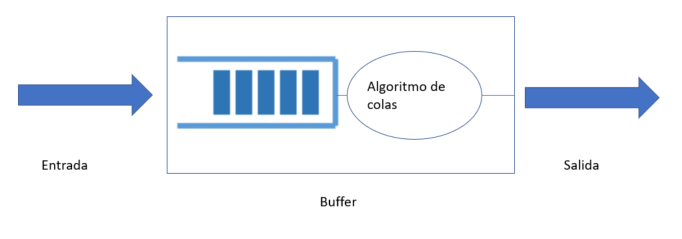
\includegraphics[width=0.7\textwidth]{img/teoriaColas.PNG}
			\caption{Esquema del funcionamiento de encolado en un \textit{router}}
			\label{teoriaColas}
		\end{figure}
		
	La teorías de colas también depende del tipo de tráfico existente en la red, existen dos casos: sin clases de tráfico internas y con clases de tráfico internas. La principal diferencia es la diferenciación que se realiza por clases, procesando de forma diferente el tráfico según el tipo de clase al que esté asociado. A continuación, se procede a detallar brevemente algunos de los algoritmos de colas más utilizados:
	
	\begin{itemize}
	    \item FIFO (\textit{First In First Out}): Este método consiste en enviar los paquetes en el orden de llegada que fueron recibidos, tal y como muestra la figura \ref{fifolifo}. Es el más utilizado, ya que es el que gran parte de los dispositivos usan por defecto.
	    \item LIFO (\textit{Last In First Out}): Al contrario que FIFO este método consiste en reordenar y enviar los paquetes en el orden inverso al que fueron llegando, ilustrado en la figura \ref{fifolifo}. Siendo el último paquete recibido el primer en ser enviado. 
	    \item PRIO: Este método tiene como base el mecanismo FIFO, no obstante lo destacable de este método es la previa jerarquización a la que son sometidos los paquetes. Primeramente, los paquetes pasan por un filtrado y acto seguido son ubicados en la cola correspondiente según su clasificación, enviando de manera más rápida los paquetes cuya prioridad es más alta. 
	\end{itemize}
	
	\begin{figure}[H]
			\centering
			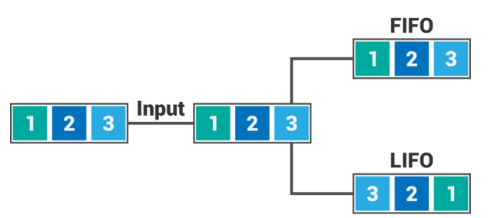
\includegraphics[width=0.7\textwidth]{img/FIFO-LIFO.png}
			\caption{Esquema del funcionamiento de las teorías FIFO y LIFO}
			\label{fifolifo}
		\end{figure}

	\subsubsection{DiffServ} 
	La arquitectura DiffServ (Servicios Diferenciados) es una arquitectura de red que permite clasificar el tráfico diferenciando según los diferentes niveles de QoS, es decir, pueden coexistir varios flujos los cuáles serán tratados y diferenciados en función del QoS. Esto se realiza con el fin de diferenciar cada tipo de tráfico del resto cçomo si de una única línea dedicada se tratase, mejorando así las prestaciones cualitativas de la red. Para entender esta arquitectura es importante introducir los términos de \textit{router} frontera (color azul) y \textit{router} núcleo de red (color naranja), la figura \ref{diffserv} muestra un escenario base que utilizaremos para explicar dichos términos y explicar su función dentro de esta arquitectura.
	
	\begin{figure}[H]
			\centering
			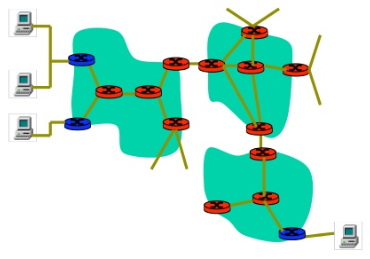
\includegraphics[width=0.5\textwidth]{img/diffserv.PNG}
			\caption{Ejemplo de arquitectura DiffServ}
			\label{diffserv}
		\end{figure}
	
	\begin{itemize}
	    \item \textit{Router} frontera: Es el encargado de hacer la clasificación de paquetes y el acondicionamiento del tráfico (\textit{shaping}/\textit{policing}). En ciertas ocasiones es deseable limitar la tasa de inyección de tráfico para algunas clases de servicios. \\
	    Tal y como muestra la figura \ref{edgerouter}, el dipositivo marca los paquetes como \textit{in-profile} en caso de que respete los términos acordados de QoS o los marca como \textit{out-profile} en caso contrario. Una vez clasificados los paquetes basándose en los valores de uno o más campos de la cabecera del paquete, se marcan diferentes categorías o clases en el campo de 8 bits \textit{Type Of Service} (ToS) de IPv4 y "clase de tráfico" de IPv6. Se usan 6 bits para identificar \textit{Differentiated Service Code Point} (DSCP) que determinan el comportamiento por salto, (PHB - \textit{Per-Hop Behavior}) que recibirá el paquete en los \textit{routers} de la red DiffServ. Los 2 bits menos significativos del campo ToS no se usan para DiffServ, sino para la notificación de congestión (ECN, \textit{Explicit Cogestion Notification}). ECN es utilizado por los extremos de una conexión TCP y los \textit{routers} intermedios que usan el algoritmo de colas RED (\textit{Random Early Detection}).
	    \begin{figure}[H]
			\centering
			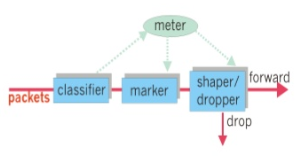
\includegraphics[width=0.5\textwidth]{img/edgerouter.PNG}
			\caption{Mecanismo de clasificación de paquetes del \textit{router} frontera}
			\label{edgerouter}
		\end{figure}
	\item \textit{Router} núcleo de red: Estos \textit{routers} no realizan el encaminado de paquetes según los campos de origen y destino, sino que realizan el encaminado en función de la marca que trae ese paquete, tratando así a todos los paquetes de igual forma. En primer lugar se encolan los paquetes recibidos basándose en las marcas que pusieron los \textit{routers} frontera, acto seguido se les da preferencia a los paquetes cuya marca es \textit{in-profile}. Cada clase de tráfico (DSCP) está asociada a un tipo de salto (PHB) que determina el tipo de tratamiento que se le va a dar al paquete. Los PHB asociados al campos DSCP se detallan a continuación:
	\begin{itemize}
	    \item EF (\textit{Expedited Forwarding}): Esta clase de tráfico recibirá el suficiente ancho de banda para equiparar o igualar la tasa mínima configurada durante un intervalo de tiempo determinado.
	    \item VA (\textit{Voice Admit}): Similar a EF sólo que añade un mecanismo de control de admisión de tráfico.
	    \item AF (\textit{Assured Forwarding}): Existen cuatro clases diferentes con los que los paquetes son clasificados por el router frontera: AF1, AF2, AF3 y AF4. Cada clase ofrece una garantía y una prioridad diferente, siendo AF1 la clase más prioritaria y AF4 la menos prioritaria.
	    \item DF (\textit{Default Group}): Tráfico \textit{Best Effort}.
	    \item CS (\textit{Class Selector}): Ofrece retrocompatibilidad y permite definir prioridades.
	\end{itemize}
	\end{itemize}
	
	\subsubsection{MPLS}
		 MPLS (\textit{Mutiprotocol Label Switching}) es un mecanismo de transporte de datos que trabaja sobre la capa de red estableciendo enlaces vrtuales entre los nodos extremo de la red MPLS. El tráfico de datos es identificado mediante una etiqueta, evitando así la necesidad de utilizar la tablas de enrutamiento IP, y asociando a cada tráfico una etiqueta en particular que define la ruta destino. Addemás, este flujo puede tener asociados diferentes parámetros de QoS. Tal y como se muestra en la figura \ref{mpls}, cada paquete tiene un camino predefinido; ese camino está definido mediante una etiqueta. Dichas etiquetas están distribuidas a los largo de la red mediante LDP (\textit{Label Distribution Protocol}). Este protocolo permite a los routers involucrados en la red, también denominados LDP \textit{peers}, intercambiar información de manera bidireccional sobre la red,  obteniendo así una base de datos LSP (\textit{Label-switched path}) sobre los diferentes caminos existentes y el tráfico existente en cada uno de ellos.
		 
		   \begin{figure}[H]
			\centering
			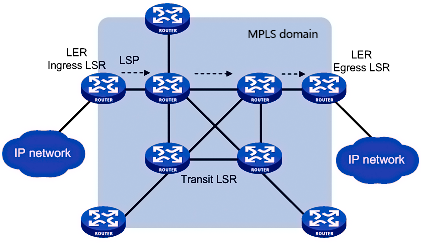
\includegraphics[width=0.5\textwidth]{img/mplsArch.png}
			\caption{Ejemplo de red MPLS}
			\label{mpls}
		\end{figure}
		 El protocolo MPLS funciona sobre tecnologías de nivel 2 como ATM, Ethernet, etc... Aparte de poder configurar la red en función a QoS, es posible realizar configuraciones VPN (\textit{Virtual Private Network}) y TE (\textit{Traffic Engineering}). El datagrama MPLS mostrado en la figura \ref{mplsData}, no es un datagrama IP convencional, si no que presenta alguna variación. Lo más destacado es el manejo de cabeceras, ya que los datagramas MPLS tienen una cabecera adicional que contiene que camino ha de tomar el paquete en cuestión. En algunos escenarios, es necesario el uso de más de una etiqueta debido a la complejidad de la red, a continuación se detallan algunos campos adicionales que son utilizados para el envío de paquetes:
		 \begin{itemize}
		    \item Etiqueta: Valor de la etiqueta MPLS.
		     \item TC (\textit{Traffic Class}): Es utilizado para identificar el tipo de QoS.
		     \item S (\textit{Bottom of Stack}): Se emplea para apilar etiquetas, cuando su valor es '1' quiere decir que es la última etiqueta.
		     \item TTL (\textit{Time To Live}): Misma funcionalidad que en otro tipo de redes, disminuye en una unidad cuando realiza un salto a lo largo de la red.
		 \end{itemize}
		 
		   \begin{figure}[H]
			\centering
			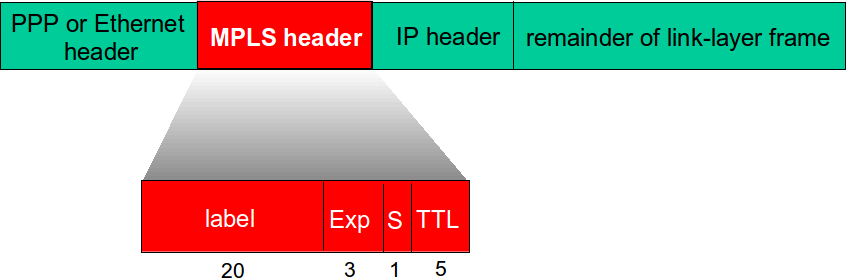
\includegraphics[width=0.5\textwidth]{img/mplsData.png}
			\caption{Representación de un datagrama MPLS}
			\label{mplsData}
		\end{figure}
		
		Al igual que los datagramas, la función y nomenclatura de los \textit{routers} involucrados en la red MPLS es diferente, ya que deben permitir reenviar paquetes utilizando las etiquetas MPLS. A continuación, se detallan los diferentes tipos de \textit{routers} involucrados en redes MPLS:
		\begin{itemize}
		    \item \textit{Ingress} LSR: \textit{Router} qeu se utiliza para acceder a la red MPLS interna. Es el encargado de añadir la primera etiqueta MPLS y realizar el reenvío correspondiente.
		    \item \textit{Intermediate} LSR: \textit{Router} ubicado en el medio de la red, debe recibir el paquete MPLS y reenviarlo al destino indicado por la etiqueta.
		    \item \textit{Egress} LSR: \textit{Router} ubicado al final de la red MPLS. Su función es desetiquetar el paquete y reenviarlo correctamente fuera de la red MPLS interna.
		\end{itemize}
		
	 La gestión de envío de los paquetes en los LSR se realiza en función de la etiqueta del paquete en cuestión y de la información contenida en la misma. En función de es información existen dos formas de recibir el paquete, por interfaz o por \textit{router}. Por un lado, si se realiza un reenvío por \textit{router} únicamente se reenvía utilizando la información de la etiqueta. Por otro lado, si utilizamos el reenvío mediante interfaz se utiliza la información existente en la interfaz del \textit{router} y la información existente en la etiqueta. En este último, cada \textit{router} puede definir su propio ámbito de etiquetas.\\
	 Aparte del uso de estas técnicas, los LSR también utilizan tablas adicionales para la gestión de reenvío de paquetes, a continuación se detallan dichas tablas:
	 \begin{itemize}
	     \item NHLFE (\textit{Next Hop Label Fordwarding Entry}): Gestiona las etiquetas de salida.
	     \item ILM (\textit{Incoming Label Map}): relaciona la etiqueta con la entrada correspondiente en la tabla NHLFE.
	     \item FTN (\textit{FEC-To-NLHFE Map}): Identifica los parámetros de una clase con la entrada correspondiente en la tabla NHLFE. Esta tabla es utilizada cuando no existe etiqueta.
	 \end{itemize}
	 Los \textit{routers} intermedios (\textit{Intermediate} LSR) deben estar sincronizados y orquestados en cuanto a las etiquetas utilizadas y protocolos durante el reenvío de paquetes, para este cometido debemos definir un protocolo que permita distribuir y realizar un control del etiquetado existente en la red. A continuación se definen los protocolos utilizados para este cometido:
	 \begin{itemize}
	     \item \textit{Label Distribution Protocol} (LDP): Este protocolo estable sesiones TCP entre los LSR involucrados para intercambiar las etiquetas que utilizarán durante el intercambio de paquetes.
	     \item \textit{Resource Reservation Protocol - Traffic Engeniering} (RSVP-TE): Es un protocolo similar a LDP, salvo que permite configurar los diferentes LSPs (\textit{Label Switch Path}) de forma explícita, ya sea total o parcial. Se define LSP como el camino unidireccional que contiene la secuencia de LSR que reenvían un paquete. Al igual que es posible establecer un LSP de forma explícita este protocolo permite añadir restricciones al mismo.
	 \end{itemize}
	 
	 \subsubsection{MPLS-TE}
	 MPLS-TE es una variación frente a MPLS que mejora el encaminamiento de paquetes mediante la implementación de LDPs y distribución de etiquetas a través de LDP. La diferencia con MPLS, y principal característica de TE, es que nos permite realizar conexiones entre nodos finales dentro de la propia red. \\\\
	 MPLS-TE utiliza el protocolo RSVP-TE para definir enlaces internos que son denominados túneles y restringen el uso de los recursos compartidos de la red a los circuitos virtual que la forman, creando así una protección mutua entre ellos. Como consecuencia de esto, la distribución del ancho de banda es igual o inferior al total disponible. Al igual que en MPLS es posible configurar los diferentes túneles en función de las propiedades de la red y las interfaces de los LSR involucrados.
	 
	 \begin{figure}[H]
			\centering
			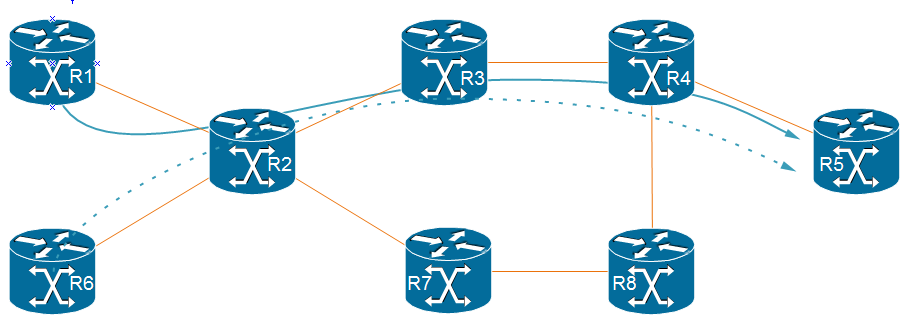
\includegraphics[width=0.5\textwidth]{img/MPLS-TE.png}
			\caption{Ejemplo de red MPLS-TE}
			\label{mplste}
		\end{figure}
		

	\section{Monitorización de redes}
	Una vez comentados los distintos protocolos de gestión de tráfico, procedemos a detallar algunos de los programas de \textit{software} libre destinados a la monitorización y gestión de redes para el desarrollo del proyecto:
	  
	\begin{itemize}
		\item Nagios Core \cite{Nagios} es un \textit{software} diseñado y desarrollado por la empresa Nagios. Permite monitorizar vía web cualquier infraestructura y dispositivo red, estableciendo un conjunto de reglas basadas en servicios y alertas reportando información sobre el funcionamiento de la red.\\
		Nagios Core ofrece gran variedad de servicios y funcionalidades respecto a la monitorización, siendo capaz de monitorizar servicios red (HTTP, SNMP, POP3, etc...) y recursos de los dispositivos (carga de CPU, temperatura, espacio libre, etc...). Igualmente, existe la opción de autoconfigurar y desarrollar nuestros propios servicios y no sólo utilizar los predefinidos por el fabricante (que aparecen por defecto). También existe la posibilidad de generar notificaciones sobre cualquier servicio, y éstas pueden ser enviadas vía email (u otro método que defina el usuario). Para una configuración personalizada no hacen falta librerías adicionales, ya que la versión Core incluye todas las funcionalidades básicas para la gestión y monitorización de redes. No obstante, se pueden incluir otras funcionalidades como representación de gráficos en un \textit{Dashboard}, exportación de configuraciones o utilización de proveedor de correo externo al de la propia herramienta. Todo esto podremos hacerlo mediante la adicción de \textit{plugins} al Core.
		
		\item Zabbix \cite{Zabbix} es un \textit{software} íntegramente libre desarrollado por Zaabix SIA. Este \textit{software} nos permite monitorizar numerosos parámetros de nuestra red, bien sean servicios (HTTP, SNMP, SSH, etc..) o bien sean parámetros de los dispositivos (uso de CPU, porcentaje uso de CPU, temperatura, etc...) referidos a los servicios y estado de los dispositivos que la componen. Para ello, Zabbix utiliza un sistema de notificaciones configurables, las cuáles pueden enviarse vía email (utilizando cualquier proveedor de correo). Dichas notificaciones nos informarán sobre los sucesos que están ocurriendo sobre los dispositivos red y los servicios configurados.\\
		En orden con lo anterior, Zabbix permite editar y configurar diferentes tipos de notificaciones y alertas sin necesidad de añadir nada a la herramienta. Además de esto, el reporte de datos es periódico y no sólo de manera numérica sino de forma gráfica (dichas gráficas también pueden ser configurables). Del mismo modo, existe la posibilidad de almacenar todo los datos reportados procedente de los dispositivos que forman la red en bases de datos (MySQL, SQLite, PostgreSQL o Oracle).
		
		\item Pandora OpenSource \cite{Pandora} es un \textit{software} de gestión y monitorización desarrollado por la empresa Pandora FMS Enterprise que proporciona una solución capaz de monitorizar cualquier infraestructura de red asegurando que todos los elementos de la red estén funcionando bajo los criterios de operación establecidos. Esto es debido a la información procedente de los dispositivos de la red al realizarse pruebas sobre ellos, ya sea de manera remota o mediante un agente. \\
		La versión libre de este software permite monitorizar y gestionar parámetros referentes a los servicios de red estándar TCP/IP y valores relacionados con el hardware de los equipos gracias a un sistema de eventos. Este sistema obtiene la información al producirse cualquier evento en la red. Al basarse en dicha funcionalidad, el usuario puede validar los eventos y agruparlos según la distribución de la red. Debido a esto el software utiliza una monitorización combinada en grupos, lo que quiere decir que, según el grupo en el que se encuentre un dispositivo, sus alertas y su configuración de servicios serán diferentes al resto.\\\\
	\end{itemize}
	
	Una vez introducidos diferentes tipos de \textit{software} en gestión y monitorización de redes procedemos a analizar cuál de ellos encaja mejor en el marco de nuestro proyecto según las diferentes limitaciones y requisitos.\\\\
	
	En primer lugar, nuestro \textit{software} debe ser capaz de monitorizar todos los requisitos mínimos para garantizar un cierto nivel de QoS. Además de esto es conveniente que exista cierta flexibilidad a la hora de modificar y añadir notificaciones en los diferentes equipos, así como la posibilidad de recibir y enviar dichas notificaciones al usuario mediante email, o cualquier método similar. Del mismo modo, el \textit{software} debe tener una integración sencilla sobre nuestra infraestructura de red.\\\\
	
	En segundo lugar, la obtención y representación de datos de forma dinámica es una parte importante que la herramienta ha de tener. Lo deseable es que la infraestructura de red sea autogestionable y plenamente monitorizable por el propio \textit{software}, es decir, tratar de que cualquier servicio y parámetro pueda ser representado de manera concreta para otorgar al usuario la información adecuada para interactuar, si fuera necesario, con la red.\\\\
	
	En tercer lugar, nuestro \textit{software} ha de ser flexible en cuanto a escalabilidad de dispositivos y configuración de notificaciones, puesto que nuestra red es extensa y heteréogenea en cuanto al número de equipos y su uso. Otro requisito a tener en cuenta es que debe cumplir con un sistema de negocio viable, ya que el proyecto tiene limitada la inversión económica y es muy deseable utilizar un software cuya prestación sea total a coste cero.\\\\
	
	Teniendo en cuenta todo lo comentado anteriormente, la solución propuesta para el proyecto es Zabbix.\\\\
	
	Zabbix permite una fácil integración y monitorización de la red, permitiendo al usuario administrar los dispositivos y configurar los servicios de manera sencilla sin excesiva complejidad. Gracias a su interfaz gráfica podemos obtener en todo momento una representacion en tiempo real del estado de los dispositivos, así como de los requisitos pertenecientes al QoS. Dichos datos pueden ser almacenados en bases de datos y exportados a ficheros.\\
	Por un lado, Zabbix no sólo permite al usuario definir dispositivos, sino que existe la posibilidad agruparlos en diferentes categorías, otorgando la opción de realizar una gestión individualizada o colectiva, según desee el usuario. Por otro lado, se pueden crear servicios mediante un fichero XML y vincularlo con el dispositivo deseado,  configurando alertas y notificaciones personalizadas. 
	